\setcounter{lstlisting}{0}
\setlength{\parindent}{0pt}
\setlength{\parskip}{\baselineskip}
%\FredComment{Do not use \textbackslash\textbackslash\ for line breaks.  Use proper paragraph breaks. If you really need no indention, you can set the parindent.}

The Halton sequence is a common low-discrepancy sequence used for Quasi-Monte Carlo simulations. It is based on the principle of using prime numbers as bases for each dimension, e.g., 2 is used for dimension 1, 3 for dimension 2, 5 for dimension 3, and so on. For each dimension, the indexes are converted from base 10 to the specific base associated with that dimension, the digits are then reversed, a decimal point is added before all the digits, and finally everything is converted back to base 10 to generate our samples.

Here is an example illustrating how Halton samples are generated:  We have a 3 dimensional Halton object and the 29th index (30th sample) would be calculated the following way:
\begin{equation}
    i = 29 = 11101_2 = 1002_3 = 104_5 \nonumber 
    \end{equation}
\begin{equation}
    11101_2 --> .10111_2 = \frac{23}{32} \nonumber
    \end{equation}
\begin{equation}
    1002_3 --> .2001_3 = \frac{55}{81}   \nonumber
    \end{equation}
\begin{equation}
    104_5 --> .401_5 = \frac{101}{125}   \nonumber
    \end{equation}
Hence our 30th sample would be \( \left( \frac{23}{32}, \frac{55}{81}, \frac{101}{125} \right) \).

Like Lattice and Sobol sequences, Halton sequences too have certain randomizations available to generate the samples. Up till now, the two randomizations of Halton implemented in QMCPy were ``QRNG''\cite{mhcl2019qrng} and ``OWEN''\cite{owen2017randomized}. ``QRNG'' uses optimized fixed permutations of the digits and also adds a random digital shift to the digits while ``OWEN'' uses independent random permutations of the digits. 
%\FredComment{Can you explain what these are?  Are they permutations of the digits?  Random start?} 

This blog discuses the implementation of three new randomizations for Halton: linear matrix scrambling (LMS), digital shift (DS), and linear matrix scrambling plus digital shift (LMS\textunderscore DS).  These randomizations are commonly used for digital nets, but have only recently been explored for Halton sequences.
%\FredComment{You need to give some motivation for why you implemented these new randomizations}
%\newline 
These new randomizations help provide unbiased estimates for QMC integration, and the variance under a linear matrix scramble is better than the variance when just using a random digital shift.  \FredComment{Is this true?}

\subsection*{LMS, DS, and LMS\textunderscore DS:}
\begin{enumerate}
    \item LMS: This stands for Linear Matrix Scrambling of Halton \cite{owen2023gain}. Based on the bases, a different scrambling matrix is generated for each dimension where the lower triangle is random between 0 and (base - 1), the diagonal is random between 1 and (base - 1), and the upper triangle has all zeros. After the indexes are converted to their base representations and a decimal point has been added before all the reversed digits, their dot product is computed with the scrambling matrix. After computing the dot product, the scrambled indexes/coefficients are converted to base 10 to generate our samples.
    \item DS: This stands for a Digital Shift. Based on the bases, a different vector is generated for each dimension which is random between 0 and (base - 1). After the indexes are converted to their base representations and a decimal point has been added before all the reversed digits, they are added to the vector and then converted to base 10 to generate the samples.
    \item LMS\textunderscore DS: This represents a combination of Linear Matrix Scrambling and a Digital Shift. The Linear Matrix Scrambling of Halton is implemented but before converting to base 10, the Digital Shift is applied to the scrambled indexes/coefficients and then conversion to base 10 occurs to generate the samples.
    \end{enumerate}
 ``LMS'' includes the origin as the first point in the sequence but ``DS'' helps prevent this, making ``LMS\textunderscore DS'' the recommended randomize option.

\subsection*{Plot examples of LMS, DS, and LMS\textunderscore DS:}
\lstinputlisting[style = Python]{LMS_DS_Halton/code.py}
   \begin{figure}[H]
    \centering
    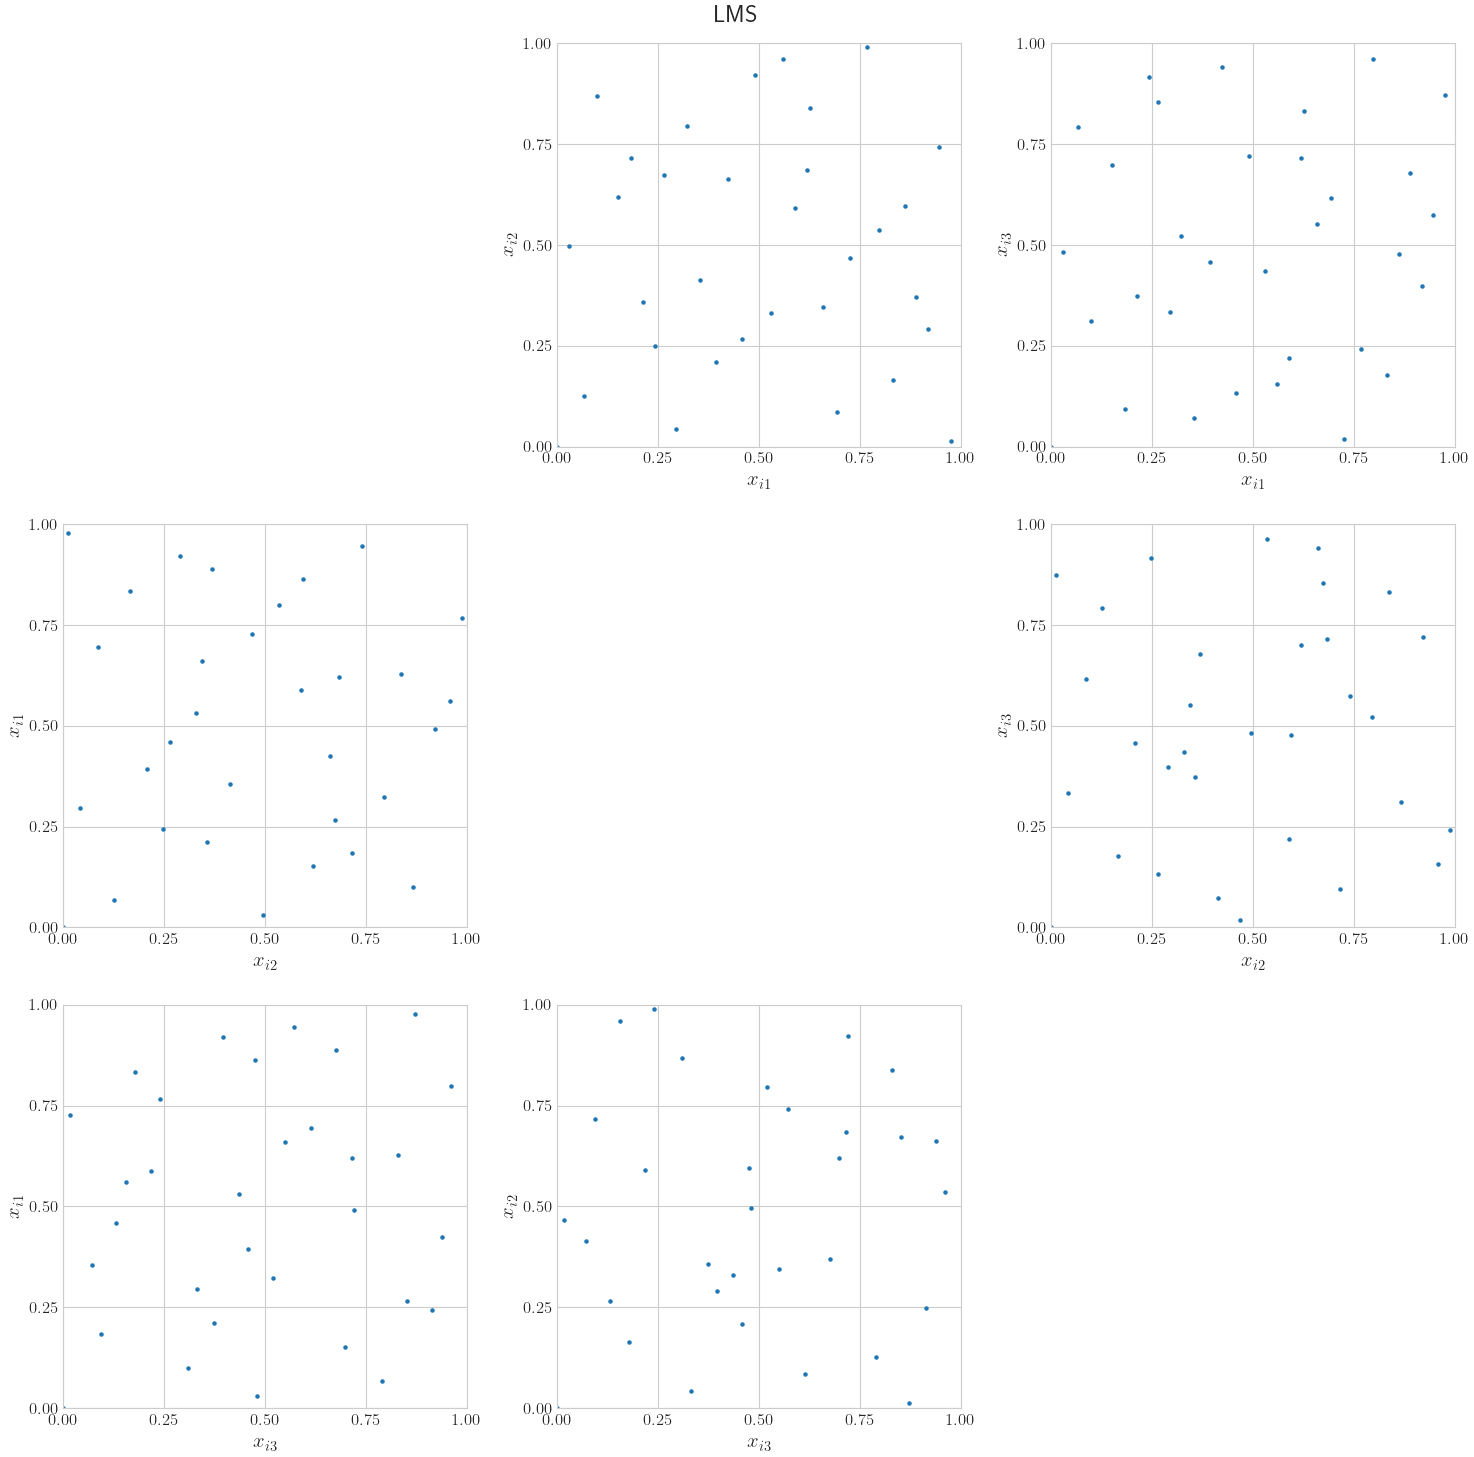
\includegraphics[width = 0.99 \linewidth]{LMS_DS_Halton/lms.png}
    \end{figure}
    \begin{figure}[H]
    \centering
    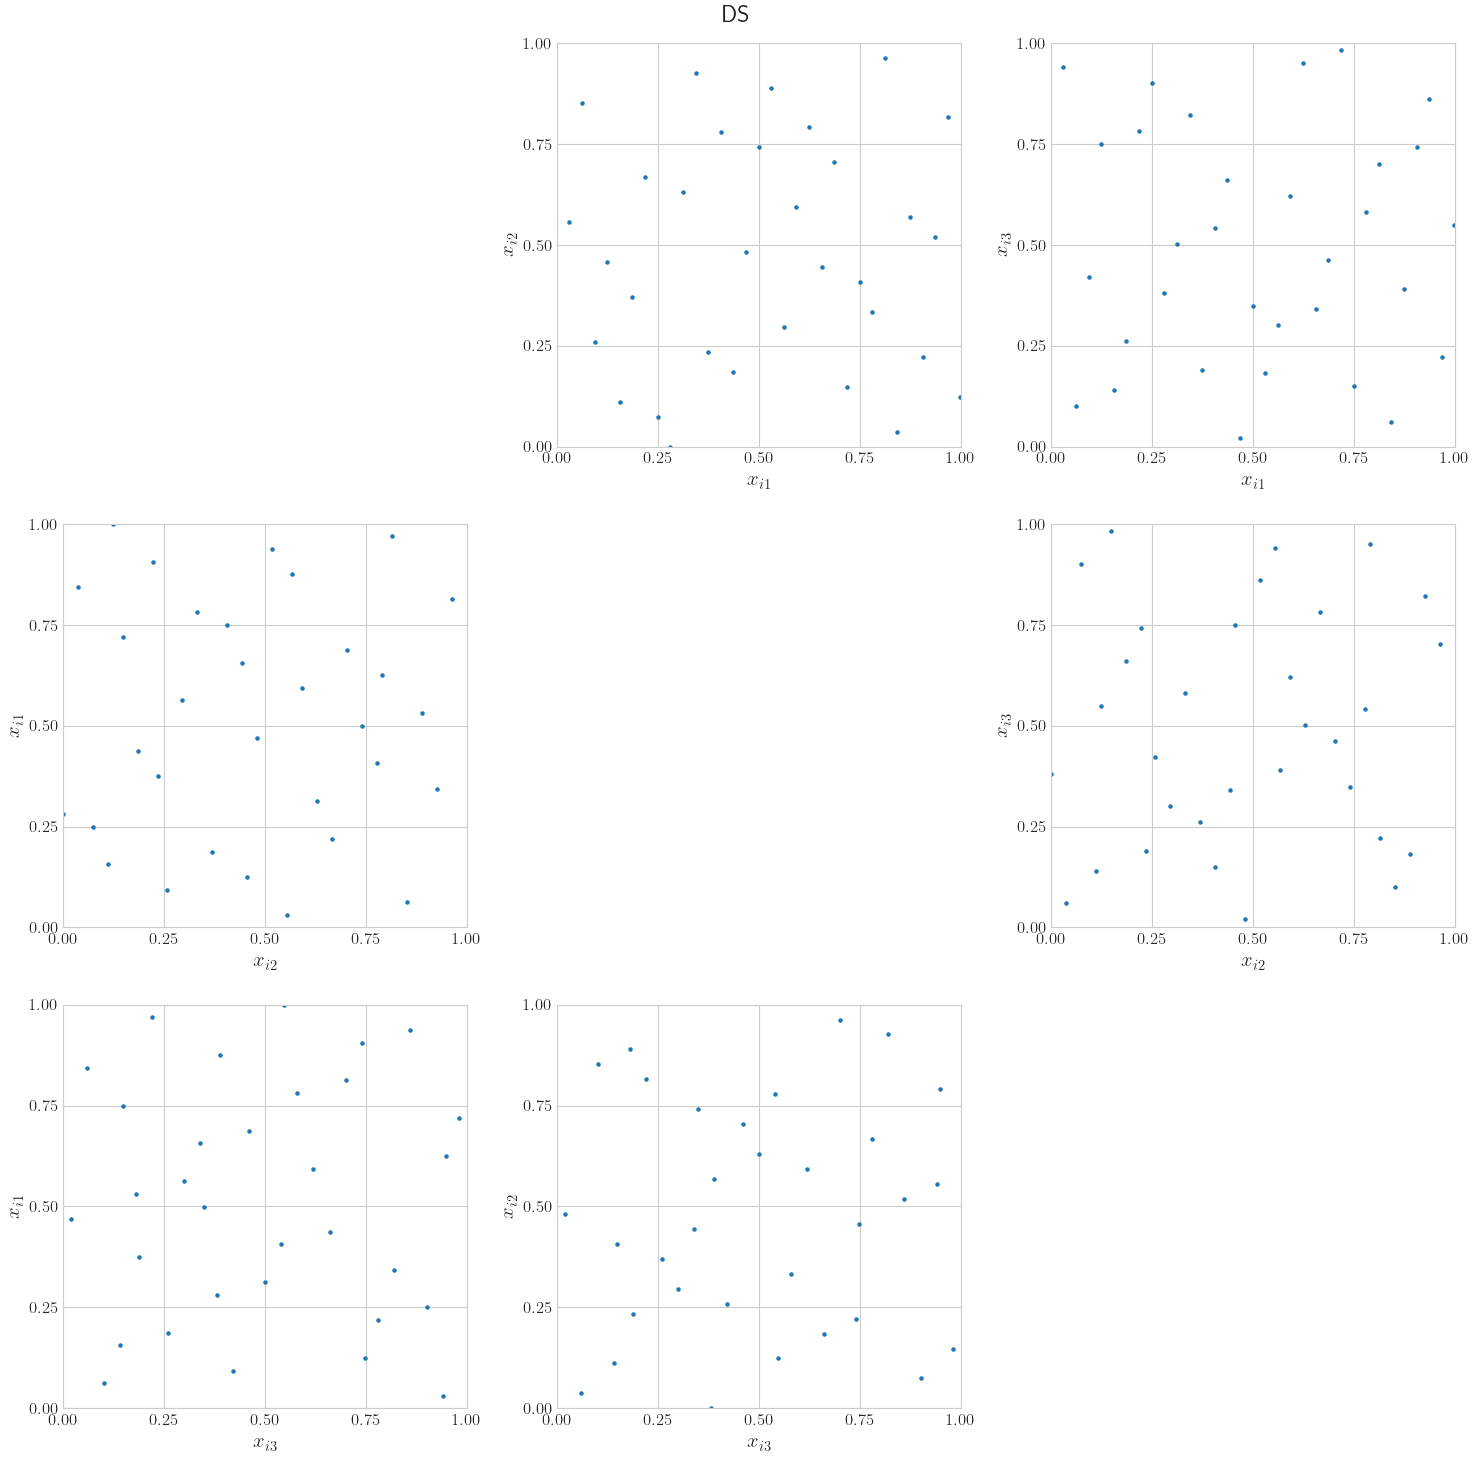
\includegraphics[width = 0.99 \linewidth]{LMS_DS_Halton/ds.png}
    \end{figure}
    \begin{figure}[H]
    \centering
    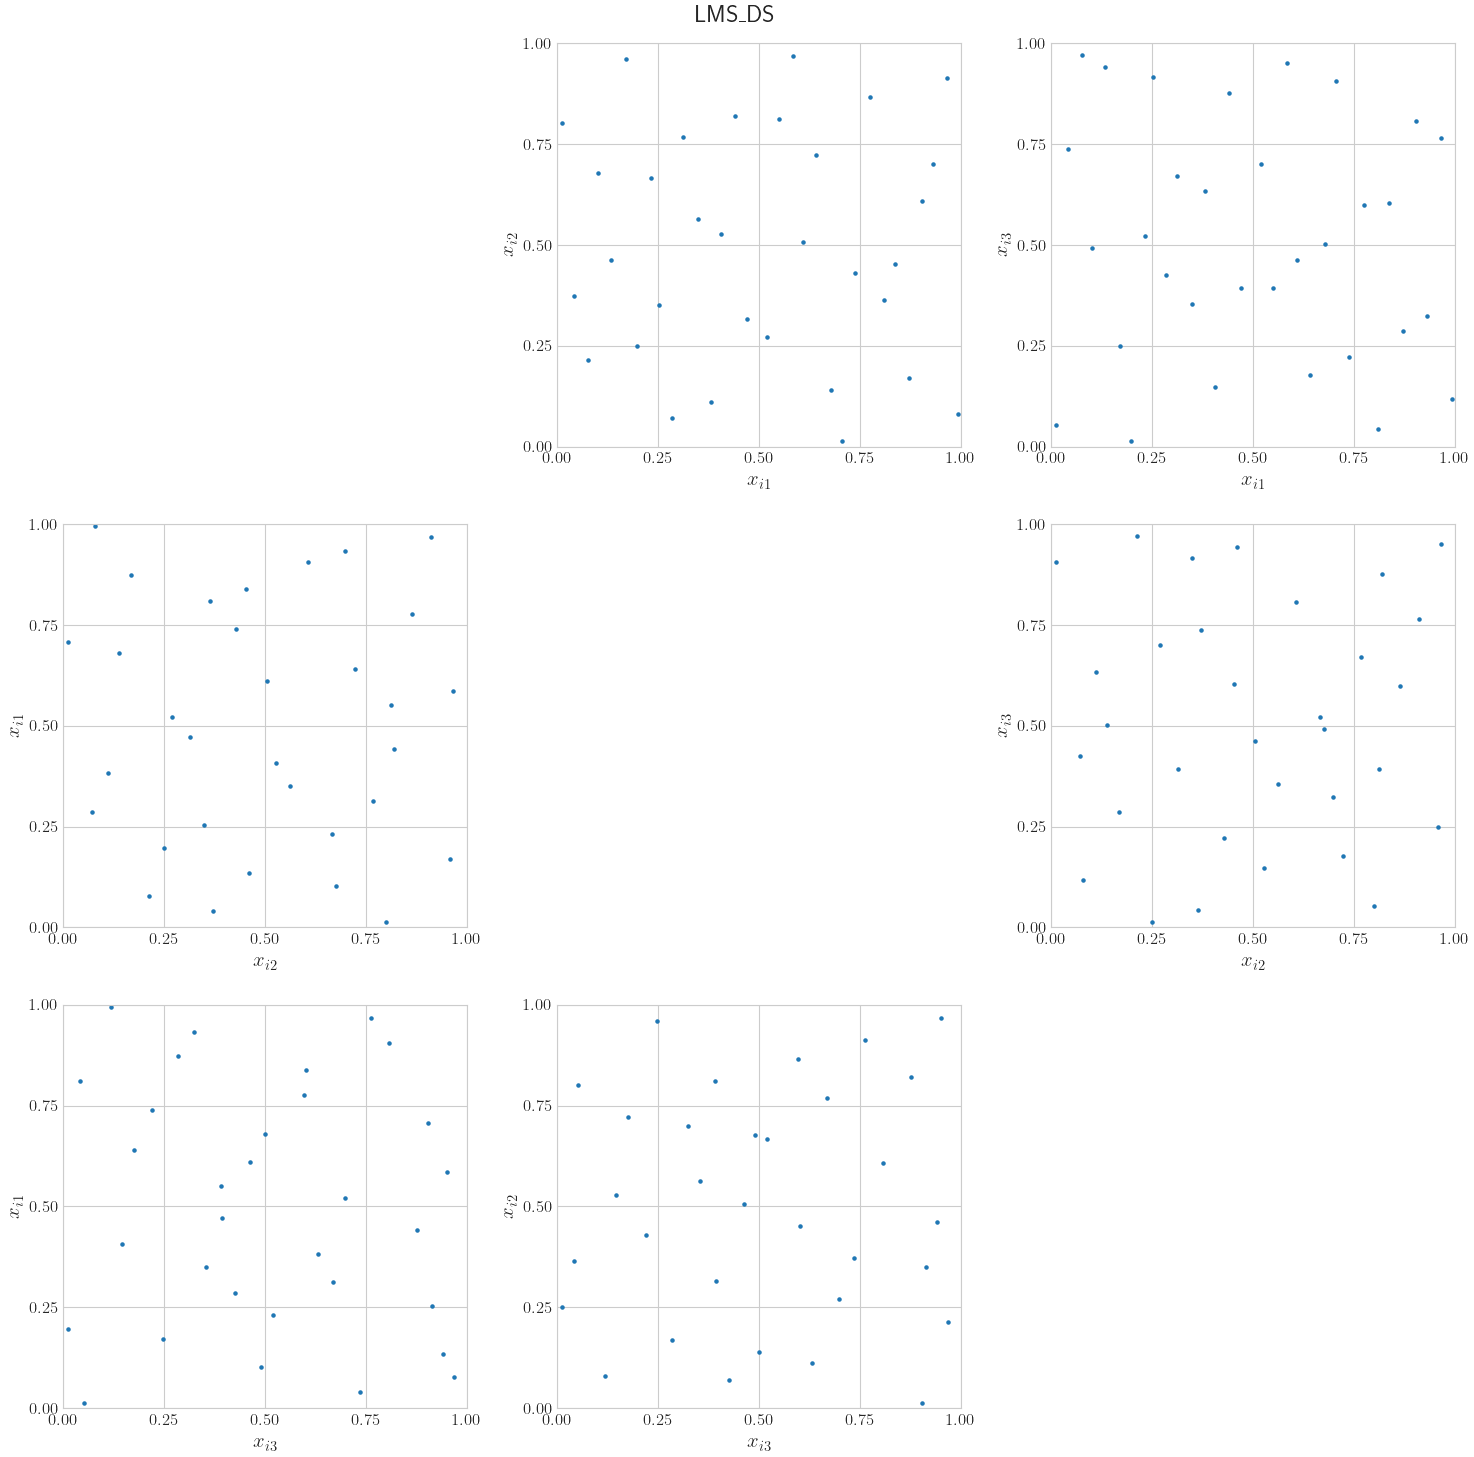
\includegraphics[width = 0.99 \linewidth]{LMS_DS_Halton/lms_ds.png}
    \end{figure}
More plot examples can be seen in the \href{https://github.com/QMCSoftware/QMCSoftware/blob/develop/demos/linear-scrambled-halton.ipynb}{Linear Matrix Scrambling and Digital Shift for Halton Notebook}.
\subsection*{Speed Comparison between all the randomization methods of Halton:}
\lstinputlisting[style = Python]{LMS_DS_Halton/comp.py}
\noindent
    \begin{minipage}{.75\textwidth}
        \lstinputlisting[caption = Speed Comparision , frame=tlrb]{LMS_DS_Halton/compare.txt}
    \end{minipage}\hfill
\newline Through this speed comparision, we can see that LMS\textunderscore DS is slower than the other randomization techniques.
\subsection*{Conclusion:}
``LMS'', ``DS'', and ``LMS\textunderscore DS'' provide us with newer ways to manipulate Halton in order to get a more variety of samples. The digital shift prevents unrandomized Halton and Scrambled Halton from including origin as the point, which allows us to use these for different True Measure objects and Integral approximations.
